% Report-Introduction.tex
% Simon Hulse
% simonhulse@protonmail.com
% Last Edited: Wed 27 Nov 2024 02:42:21 PM EST

% !TeX root = ./Report-Body.tex
\chapter{Introduction}

% Introduction text goes here
NMR Spectroscopy has been widely used for the study of biomolecular systems for over 70 years. The importance of the technique is evidenced by the fact that 2 Nobel Prizes in Chemistry have been awarded to pioneering figures in NMR (Ernst, 1991 and W\"{u}thrich, 2002). At present, it is the only experimental method that can measure both the structure and dynamics of biomolecules at atomic resolution on varying timescales.  Despite the unique information NMR can offer, there are certain features which limit the size of molecules that can feasibly be studied using it. As the size of the molecule increases, so too does the number of distinct chemical environments. This leads to increased spectral crowding, which can make the resolution of individual environments challenging. On top of this, the detectable magnetisation emanating from a molecule decays - via a process called \textit{relaxation} - more rapidly with increasing molecular size, which further reduces the resolving power of the experiment.\\
There are relatively few solved structures of biomolecules with molecular masses greater than 25 kDa using conventional techniques\cite{RN14}. Since 1997, development of \textit{Transverse Relaxation Optimised SpectroscopY} (TROSY) has enabled studies of molecules far larger. The original TROSY methodology was developed to target scalar-coupled $^{15}$N-$^1$H pairs commonly encountered in proteins\cite{RN15}. Additional TROSY techniques have been developed since, including methyl-TROSY, which involves probing proteins that have been selectively labelled with $^{13}$C methyl groups\cite{RN17, RN37}. This particular innovation allows biomolecules up to 1MDa to be studied\cite{RN16,RN35,RN36,RN22}. Despite this, the possibility of studying even larger systems, such as membrane-bound proteins, is of course desirable. The aim of this thesis is to explore possibilities for the development of such methods.\\
The use of $^{19}$F NMR may be a step towards extending the limits of bimolecular NMR. Whilst fluorine does not exist naturally within biomolecules, methods allowing the incorporation of $^{19}$F nuclei into proteins are emerging\cite{RN19}. The $^{13}$CF$_3$ group has certain features that make it a promising target for TROSY experiments. Firstly, the only $^{19}$F environments within a protein would come from the selectively inserted $^{13}$CF$_3$ labels, and therefore the resultant spectra would be far less crowded. Furthermore, the relaxation behaviour of $^{13}$CF$_3$ should vary substantially from $^{13}$CH$_3$, giving rise to the possibility of developing new NMR experiments that exploit this. The primary reason for this difference stems from the typically large $^{19}$F \textit{chemical shift anisotropy} (CSA), which arises due to a non-uniform electron density about the nucleus.\\
Whilst most NMR experiments can be adequately understood without a detailed appreciation of relaxation, this isn't the case for the TROSY experiments. The method is based on being highly selective about generating certain magnetisations that have favourable relaxation properties. The major focus of this thesis is to investigate the theory of relaxation in I$_3$S spin-systems, freely rotating as a part of larger molecules. Subsequently, validation of this theory via experimental means is attempted. Armed with a detailed understanding of I$_3$S relaxation phenomena, it will then become possible to devise an optimal $^{13}$CF$_3$-TROSY experiment.
\section{Basics of NMR and Relaxation} \label{sec1.1}
NMR experiments involve perturbing the magnetisation associated with an ensemble of spins away from its equilibrium state. This is achieved by the application of radio-frequency (rf) pulses. After such a perturbation is applied, the sample's net magnetisation will eventually return back to equilibrium, via relaxation. As a simple illustration of relaxation, one can consider how a sample's magnetisation evolves with time using the \textit{vector model}\cite{RN39}.\\ Consider an ensemble of isolated spin-$\frac{1}{2}$ nuclei, subjected to an external magnetic field, $\vec{B_0}$. The ensemble's net magnetisation, described by $\vec{M}$, will be parallel $\vec{B_0}$ at equilibrium. It is possible to rotate the net magnetisation of the sample into the plane perpendicular to the field direction. This is achieved by the application of a $\ang{90}$ rf pulse. Subsequently, $\vec{M}$ precesses about $\vec{B_0}$. However, the magnetisation does not precess within this perpendicular plane indefinitely. Instead, it gradually reverts back to its equilibrium position. Two separate relaxation rates are important to note:
\begin{itemize}
\item \textit{Longitudinal Relaxation}: the restoration of magnetisation along the field-direction (conventionally the z-direction), involving a change in population of spin states.
\item \textit{Transverse Relaxation}: a loss of coherence between spins, leading to depletion of magnetisation in the plane perpendicular to the field-direction. This does not require a change in population of the spin states.
\end{itemize}
\begin{figure}
\centering
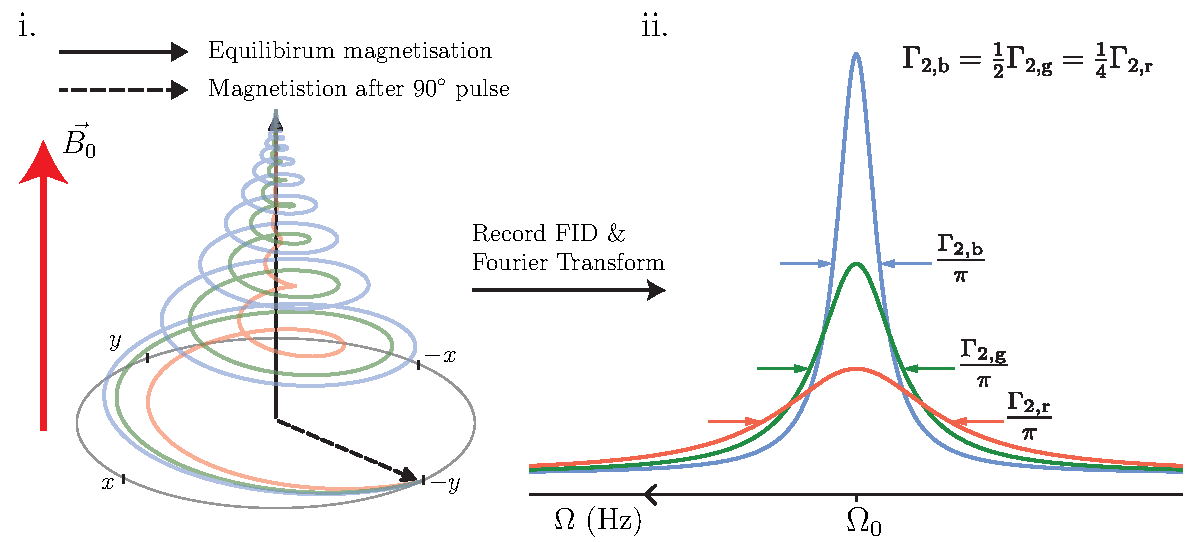
\includegraphics[scale=0.75]{./Figures/SimonsFigs/relaxation.pdf}
\caption{i. The time evolution of the bulk magnetisation for a system of spin-$\frac{1}{2}$ nuclei after a $\ang{90}$ pulse, described by the vector model. The relaxation of the magnetisation is parametrised by the longitudinal and transverse relaxation rate constants, $\Gamma_1$ and $\Gamma_2$. The three coloured spirals illustrate the time evolution of the magnetisation vector $\vec{M}$, with differing $\Gamma_2$ values, red having the largest value and blue having the smallest value. $\Gamma_1$ is kept constant for all cases. ii. The resulting signal, detected in the transverse plane, is Fourier Transformed to produce a spectrum, whose linewidth at half the peak's maximum intensity is $\frac{\Gamma_2}{\pi} \si{\myhertz}$}
\label{VecMod}
\end{figure}
These two processes typically occur at different rates in aqueous solution, parametrised by $\Gamma_1$ and $\Gamma_2$, respectively. Figure \ref{VecMod}.i illustrates how the magnetisation of an ensemble of spin-$\frac{1}{2}$ nuclei evolves with time, using the vector model. In the \textit{rotating frame}\cite{RN6}, the $x$-, $y$- and $z$-components of the magnetisation are described as follows:
\begin{equation}
M_x(t) = |\vec{M_0}| \sin(\Omega_0 t) e^{-\Gamma_2 t} \hspace{10pt} M_y(t) = -|\vec{M_0}| \cos(\Omega_0 t) e^{-\Gamma_2 t} \hspace{10pt} M_z(t) = |\vec{M_0}|\left(1 - e^{-\Gamma_1 t}\right)
\end{equation}
where $|\vec{M_0}|$ is the magnitude of the equilibrium magnetisation vector, and $\Omega_0$ is the offset frequency, equal to $\omega_0 - \omega_{\text{rf}}$. These expressions give rise to the spiral-like path that the magnetisation vector follows as it returns to equilibrium in Figure \ref{VecMod}.i. An NMR spectrometer is set up such that it is able to detect magnetisation transverse to the field direction. The signal it detects, called the free induction decay (FID), is Fourier Transformed to convert it from the time domain to the frequency domain. The resulting spectrum consists of a single peak, described by a Lorentzian function:
\begin{equation}
S(\Omega) = \text{Re}\left(\int \limits_0^{\infty} \underbrace{(M_x(t) + iM_y(t))}_{e^{i\Omega_0 t}}e^{-\Gamma_2 t}e^{i \Omega t} dt \right) = \frac{\Gamma_2}{\Gamma_2^2 + (\Omega_0 - \Omega)^2}
\end{equation}
The transverse relaxation rate constant, $\Gamma_2$ has a direct impact on the width of the peak, Figure \ref{VecMod}.ii. By noting that the maximum peak intensity occurs at $\Omega_0$,
\begin{equation}
\label{eq1.4}
S_{\text{max}}=S(\Omega_0)=\frac{1}{\Gamma_2} \therefore\  S_{\text{half-height}} = \frac{1}{2\Gamma_2}  \implies \Omega_{\text{half-height}} = \Omega_0 \pm \Gamma_2
\end{equation}
Hence, the width of a peak at half it's maximum is given by $2\Gamma_2\ \si{\radian\per\second} = \frac{\Gamma_2}{\pi}\ \si{Hz}$. The smaller $\Gamma_2$ is, the more intense and sharper the resultant spectral peaks will be.\\
Relaxation of the signal that is ultimately detected isn't the only factor that impacts the sensitivity of NMR experiments. Most NMR pulse sequences utilise several rf pulses, along with very precisely defined delay periods, on coupled spin systems. During the sequence, various forms of magnetisation are generated, which are used to provide detailed insights into molecular structure and function. But as the pulse sequence occurs, the magnetisation is constantly relaxing. This is particularly detrimental for large macromolecules that tumble very slowly in solution, as signal relaxation is typically very fast. By the time of acquisition, the manipulated magnetisation may have such a small intensity that it is indistinguishable from the stochastic noise inherent to all spectra. For these large systems, it is paramount to be highly selective in choosing the magnetisations that are allowed to evolve during the pulse sequence. This is precisely the aim of TROSY.
\section{An Overview of TROSY}
All TROSY experiments are devised with the same objective: to find a pulse sequence that takes at least some of the sample's magnetisation along a pathway where it is slowly relaxing at all times. I outline the key principles of two well-established TROSY techniques below. It is envisaged that combining traits of both of these experiments (notably dipolar/CSA interference from one, and dipolar/dipolar interference from the other) will yield a highly effective technique for targeting $^{13}$CF$_3$ moieties.
\subsection{$^{15}$N-$^1$H TROSY}
$^{15}$N-$^{1}$H spin pairs in proteins, excluding contributions from external spins, experience two major spin-relaxation mechanisms. The first of these is a dipolar interaction between the two nuclei. Secondly, there is a considerable $^{15}$N CSA. Both interactions average to zero during the measurement time-scale, but their fluctuations, induced by molecular tumbling, dominate relaxation. A one-dimensional $^1$H spectrum of a single $^{15}$N-$^{1}$H moiety will have a doublet structure as a result of scalar coupling between the nuclei. A doublet would also be observed if a 1D $^{15}$N spectrum was acquired. For each resonance in these doublets, the relaxation behaviour will differ. Notably, for resonances where the two major mechanisms reinforce each other, relaxation will be particularly fast, corresponding to a large $\Gamma_2$ value. Conversely, resonances in which these mechanisms act in opposite senses will relax slowly. As a result, the line widths of the peaks within each doublet will be different. Small, rapidly tumbling molecules do not show much discrepancy in peak widths within a doublet. By contrast, large, slowly tumbling molecules will typically exhibit drastic differences in peak widths, Figure \ref{NHTrosy}.\\
\begin{figure}
\centering
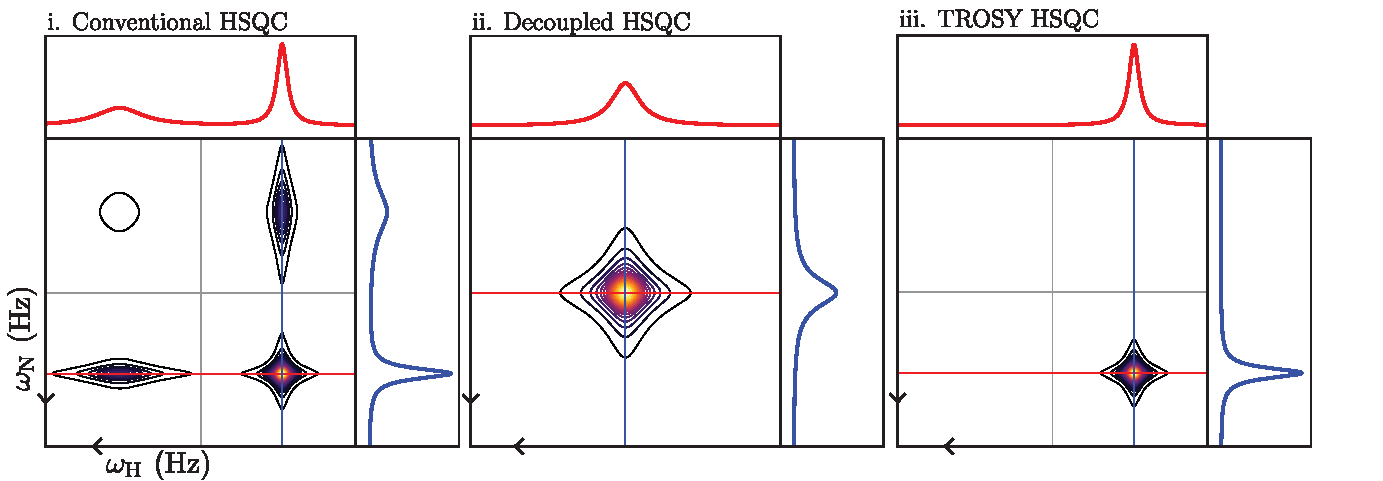
\includegraphics[scale=0.7]{./Figures/SimonsFigs/NHTrosy.pdf}
\caption{i. A HSQC spectrum of a typical $^{15}$N-$^1$H moiety in a large protein will feature peaks with highly pronounced linewidth differences, as a result of relaxation interference effects. ii. Decoupling such spectra produces peaks that originate from signal which has slowly and rapidly relaxing magnetisations mixed together, and can give rise to relatively low intensity peaks as a result. iii. In a $^{15}$N-$^1$H TROSY experiment, the use of phase-cycling discards signal that is rapidly relaxing, and retains the slowly relaxing signal only.}
\label{NHTrosy}
\end{figure}
A $^{15}$N-$^{1}$H Heteronuclear Single Quantum Coherence (HSQC) experiment produces a two-dimensional spectrum, with proton chemical shift on one axis, and $^{15}$N shift on the other. The resultant peaks provide correlations between scalar coupled $^{15}$N-$^{1}$H pairs. In the $^{15}$N-$^1$H TROSY experiment, selection of the peak corresponding to slowly relaxing magnetisaions in both dimensions is achieved via phase-cycling. The result is a loss of total signal obtained from an NMR experiment, though the signal retained gives rise to an intense, sharp line, Figure \ref{NHTrosy}.iii. For sufficiently slowly tumbling molecules, with inherently fast-relaxing magnetisations, intensity gains relative to conventional decoupled spectra are achieved using this methodology.
\subsection{Methyl TROSY}
\begin{figure}
\centering
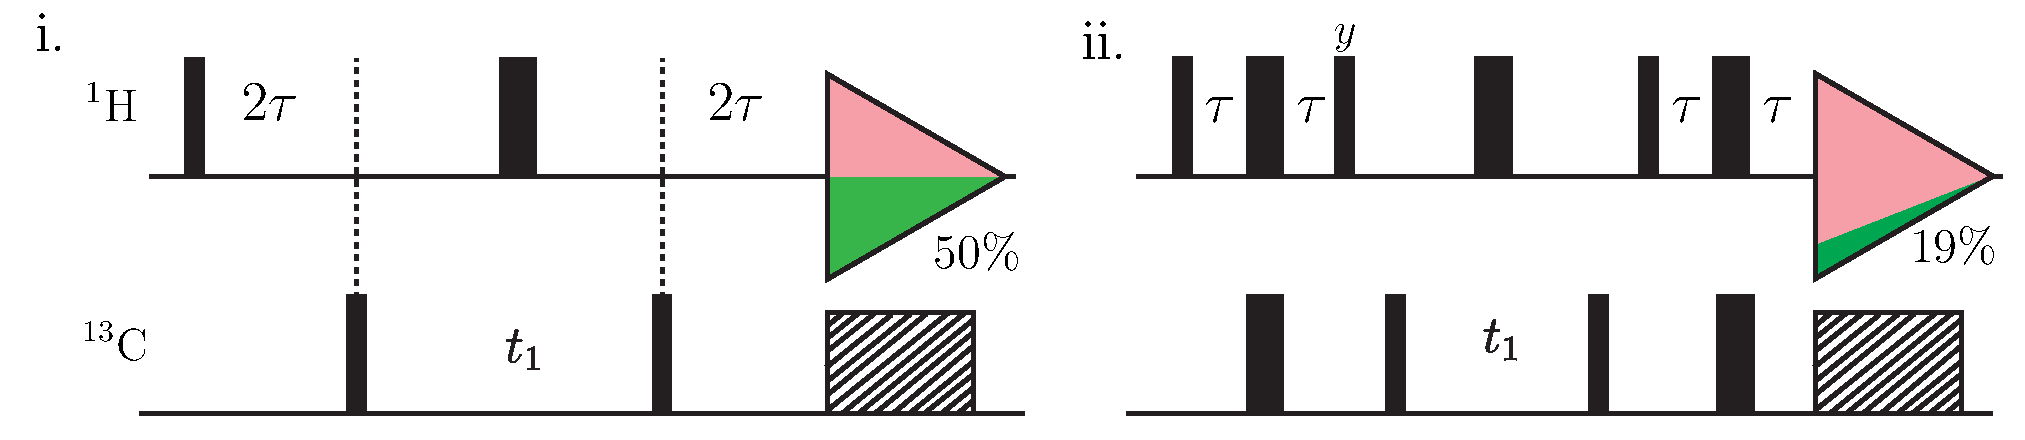
\includegraphics[scale=0.4]{./Figures/SimonsFigs/HSQCHMQC.pdf}
\caption{Simplified pulse sequence diagrams for a HMQC and a HSQC experiments (i. and ii. respectively). Narrow (Wide) bars represent $\ang{90}$ ($\ang{180}$) rf pulses, applied to the nucleus specified. The detected signal (FID) is represented by a triangle. During detection of the FID, heteronuclear decoupling (represented by a dashed box) is applied to the $^{13}$C nucleus to remove multiplet structures. The optimum value of the time $\tau$ is $\frac{1}{4J_{\text{CH}}}$, where $J_{\text{CH}}$ is the $^{13}$C-$^1$H scalar coupling constant.}
\label{HSQCHMQC}
\end{figure}
Within the $^{13}$CH$_{3}$ moiety, relaxation is dominated by numerous dipolar interactions (those being $^{13}$C-$^1$H and $^1$H-$^1$H dipolar interactions). The HSQC experiment is very poor for the study of methyl groups in large macromolecules, as during the pulse sequence, rapidly and slowly magnetisations are heavily mixed via the application of numerous $\ang{90}$ rf pulses. The Heteronuclear Multiple Quantum Coherence (HMQC) experiment, remarkably, is an optimal TROSY experient for methyl groups\cite{RN17, RN37}, Figure \ref{HSQCHMQC}. For the case of large macromolecular systems, on the order of hundred of $\si{\kilo\dalton}$ and above, calculations show that 50\% of the total signal detected from a HMQC experiment originates from magnetisation that is slowly relaxing throughout the pulse sequence. This is the case for only 19\% of the detected signal in a HSQC experiment\cite{RN17}.
\section{Thesis Outline}
In the the next chapter of this thesis, models used to describe relaxation phenomena in I$_3$S spin-systems are derived, which are extensions of current models used. The models presented have the benefit of being appropriate for all molecular size regimes. As well as this, they incorporate all appropriate relaxation mechanisms, including the I-spin CSA, which is crucial for the case of $^{13}$CF$_3$ spin systems. Following a derivation of the theory, theoretical calculations of selected relaxation rates are presented, and analysed in detail. From this, predictions on the viability of a $^{13}$CF$_3$ moiety as a good candidate for a TROSY methodology are made. Finally, some experimental relaxation studies on a system intended to mimic the behaviour of biomolecules are presented, in attempts to validate our proposed theory.
